\chapter{Quá trình Markov}
\label{ch:02}
	Chương này trình bày định nghĩa, một số ví dụ về Xích Markov và Quá trình Markov. Kiến thức của chương được tổng hợp từ tài liệu \cite{Gagniuc2017}.
\section{Xích markov}
\begin{dn} \rm
Cho không gian trạng thái $E$,$\lbrace S_{t}\rbrace _{t\geq 0}$ được gọi là một xích Markov nếu nó thỏa mãn tính không nhớ:
\begin{align}
P(S_{t+1}=s_{t+1}|S_{t}=s_{t},S_{t-1}=s_{t-1},...,S_{0}=s_{0}) = P(S_{t+1}=s_{t+1}|S_{t}=s_{t}),
\end{align}
với $t\in \mathbb{N}$ và $s_{i} \in E, i = 0,1,...,t+1.$
\end{dn}

\begin{vd}
Xích Markov các trạng thái của một sinh viên trong lớp với xác suất chuyển được minh họa như hình \ref{h2.1}. 
\begin{itemize}
\item Tập không gian trạng thái $S = \lbrace FB,C,Pt,Sl \rbrace $ tương ứng với các hoạt động Facebook, Class, Party và Sleep của sinh viên.
\item Ma trận xác suất chuyển:
\begin{align*}
\begin{bmatrix}
0.9&  0.1&  0& 0\\ 
0.5&  0&  0.4& 0.1\\ 
0&  0.5& 0 & 0.5\\ 
0 & 0 & 0 & 1
\end{bmatrix}
\end{align*}
\end{itemize}
\newpage
\begin{figure}[ht] {\label{h2.1}}
    \centering
    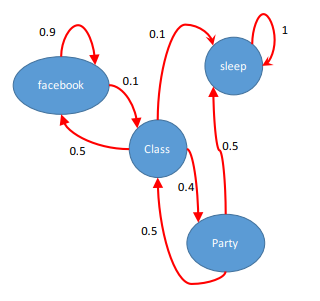
\includegraphics[scale=0.7]{vidumarkovchain.png}
    \caption{Sơ đồ chuyển trạng thái của sinh viên.}
    \label{fig:tactumoitruong}
\end{figure}
\end{vd}
\section{Quá trình Markov}
\begin{dn} \rm
$\lbrace S_{t}\rbrace _{t\geq 0}$ với không gian trạng thái hữu hạn $E$ được gọi là quá trình Markov nếu thỏa mãn :
\begin{align}
P(S_{t+s}=j|S_{u};u\leq t)=P(S_{t+s}=j|S_{t}).
\end{align}
\end{dn}
\begin{nx} \rm
Nếu $Pr(S_{t+s}=j|S_{t}=i)=Pr(S_{s}=j|S_{0}=j)$ thì quá trình Markov này được gọi là quá trình Markov dừng.
\end{nx}